\chapter{Untersuchung von MorphNet}\label{sec:morphexperimente}

Die in Kapitel \ref{sec:morphnet} erläuterte Methode zum ``schnellen Ressourcen beschränkten Strukturlernen'' (MorphNet) wird in diesem Kapitel evaluiert. In Algorithmus \ref{alg:morphnet} wird das Vorgehen von MorphNet mittels Pseudocode dargestellt. Im ersten Schritt zur Evaluierung werden die einzelnen Schritte in diesem Algorithmus evaluiert. Im zweiten Schritt wird dann überprüft, wie gut der Algorithmus mit den in Kapitel \ref{sec:konzept} genannten Rahmenbedingungen abschneidet. Da für ide Untersuchung der einzelnen Schritte von MorphNet die Ausführungszeit unwichtig ist wird dieser Teil auf der Geforce GTX 1080 Ti ausgeführt.

\section{Evaluierung der einzelnen Schritte von MorphNet}
Im ersten Schritt von MorphNet wird das Netz trainiert um 
\begin{equation}
\mathcal{W}^{\ast}=\underset{\mathcal{W}}{arg min}\; l(f(\mathbf{x_i}, \mathcal{W},y_i) + \lambda \mathcal{G}(\mathcal{W}))
\end{equation}
zu finden. Der Regularisierer $\mathcal{G}$ ist in dieser Formel dafür zuständig, dass die gewählte Zielgröße minimiert wird. Die zwei möglichen Zielgrößen sind die Modellgröße und Anzahl an FLOPs. Für beide Zielgrößen gilt, dass die im Regularsierer verwendete Formel nur eine vereinfachte Form der Zielgrösse berechnet. 
Zunächst wird evaluiert, welchen Effekt der Regularisierer auf die Zielgröße hat. Dabei werden nur die ersten beiden Schritte des MorphNet-Algorithmus durchgeführt.
In Abbildung \ref{abb:morphFLOPs} ist in Grün abgebildet, wie sich der Wert des Regularisieres für die Zielgrösse FLOPs während dem Training verändert. Die blaue Kurve in Abbildung \ref{abb:morphFLOPs} ist der tatsächliche Verlauf der Flops über die Trainingszeit. Die blaue Kurve wird in Schritten weniger, da das Netz nur alle fünf Epochen mittels der zweiten MorphNet-Schrittes kleiner wird. Die verzögerte Reduzierung der Zielgröße liegt daran, dass erst mit einer gewissen Anzahl entfernbarer Gewichte ttsächlich eine Änderung an den FLOPs passiert. Für die Zielgröße Modellgröße ist der Verlauf der beiden Kurven in Abbildung \ref{sec:morphSize} abgebildet. Für die Zielgröße Modellgröße muss $\lambda$ größer sein um einen Effekt auf die Zielgröße zu haben.

\begin{figure}
     \centering
     \subfloat[][]{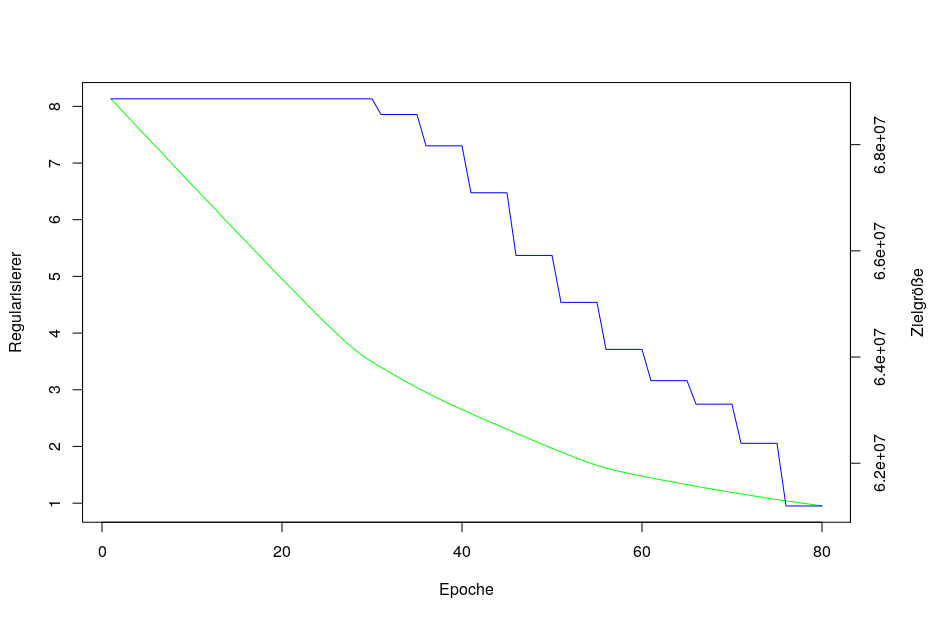
\includegraphics[width=0.47\textwidth]{KapitelPartB/Images/morph1.png}\label{abb:morphSize}}
     \hfill
     \subfloat[][]{
     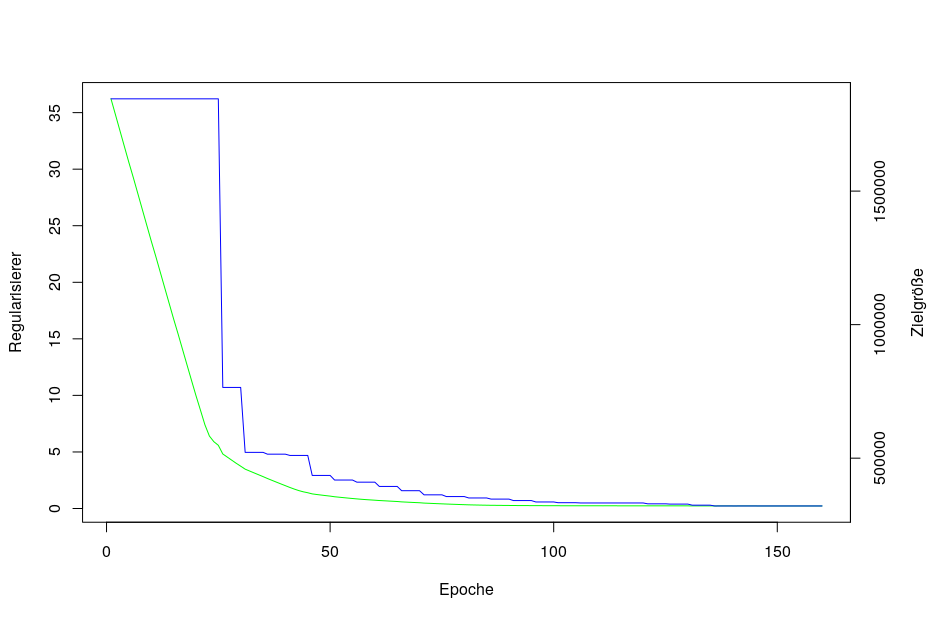
\includegraphics[width=.47\linewidth]{KapitelPartB/Images/morph2.png}\label{abb:morphFLOPs}
     }
     \caption{Vergleich Zielgröße mit Wert des Regularisierers für (a) FLOPs (b) Modellgröße }
     \label{abb:morph1}
\end{figure}

Der Effekt von verschieden großen $\lambda$ wird im nächsten Schritt untersucht. Zu diesen Zweck wird ein Netzwerk mit verschiedenen Werten für $\lambda$ trainiert. Auch hier werden nur die ersten beiden Schritte des MorphNet-Algorithmus mehrfach hintereinander durchgeführt. In Abbildung \ref{abb:morphFlops1} ist zu sehen, wie sich der Morph-Net Algorithmus bei verschiedenen $\lambda$ für die Zielgröße FLOPs verhält. 


Dabei wird das Netz jeweils für fünf Epochen trainiert und anschliessend wird das Netz beschnitten. Abhängig von der Größe von $\lambda$ wird dem Regularisierer mehr oder weniger Gewicht gegeben. Dies sorgt für eine unterschiedlich große Verkleinerungsrate. In Abbildung \ref{abb:morphSize1} ist abgebildet wie sich die Netzverkleinerungsraten verändern, bei der Zielgröße Modellgröße.  

\begin{figure}
     \centering
     \subfloat[][]{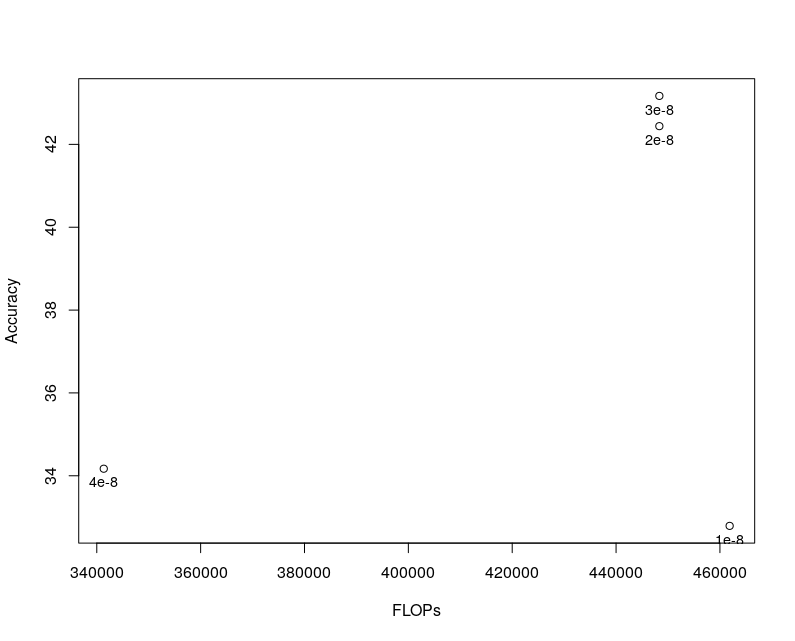
\includegraphics[width=0.47\textwidth]{KapitelPartB/Images/morph3.png}\label{abb:morphFlops1}}
     \hfill
%     \subfloat[][]{
%     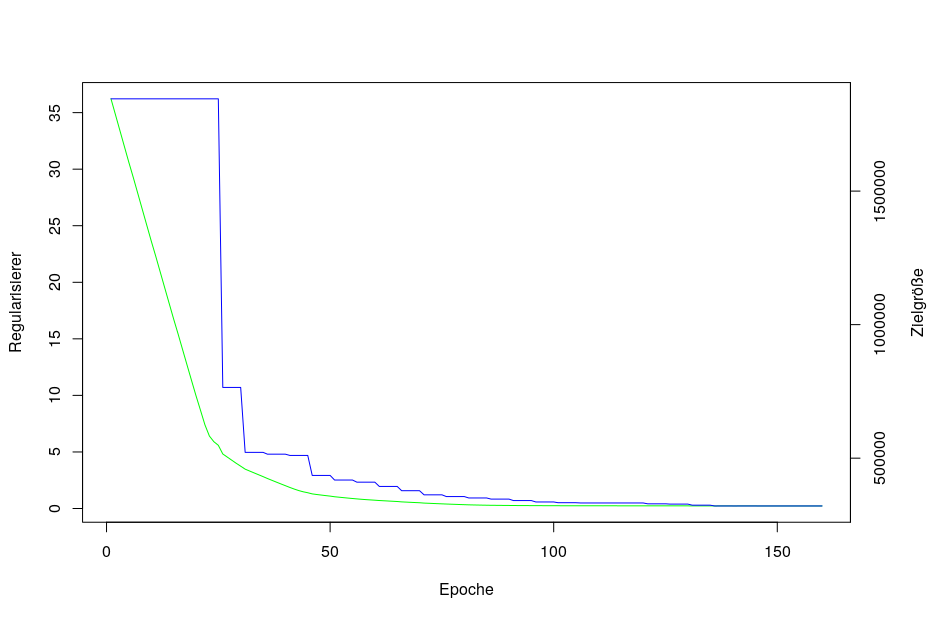
\includegraphics[width=.47\linewidth]{KapitelPartB/Images/morph2.png}\label{abb:morphSize1}
%     }
     \caption{Effekt verschieden großer $\lambda$ auf  (a) FLOPs (b) Modellgröße }
     \label{abb:morph2}
\end{figure}
Im letzten Schritt wird evaluiert, welchen Effekt die verschiedenen $\lambda$ auf den gesamten MorphNet-Algorithmus haben. Auf Grund dieser Ergebnisse werden die Parameter von MorphNet ermittelt, welches im nächsten Unterkapitel mit den Rahmenbedingungen von Kapitel \ref{sec:konzept} evaluiert wird.



\section{Evaluierung der Ergebnisse von MorphNet}

Die in Kapitel \ref{sec:konzept}  vorgestellte Vorgehensweise wir hier verwendet, um MorphNet zu evaluieren. Dies bildet die Grundlage zum Vergleich in Kapitel \ref{sec:vergleich}.














\chapter{Vergleich}\label{sec:vergleich}

\begin{comment}
\chapter{Additive Verfahren}

\subsection{Zahlenformate}\label{sec:zahlen}
\todo[inline]{Text fertig schreiben; etwa 4 Stunden}
\begin{itemize}
 \item FP16 bereits probiert
\end{itemize}


FP16 nur auf RTX 2080 sinnvoll
Bietet nach erster Messung etwa 28 \% Prozent Gewinn.

Code für dieses Verfahren liegt vor: Amp apex von Nvidia

AMP bietet 3 mögliche Optimierungsstufen:

O1
Patch all Torch functions and Tensor methods to cast their inputs according to a whitelist-blacklist model. Whitelist ops (for example, Tensor Core-friendly ops like GEMMs and convolutions) are performed in FP16. Blacklist ops that benefit from FP32 precision (for example, softmax) are performed in FP32. O1 also uses dynamic loss scaling, unless overridden.

02
casts the model weights to FP16, patches the models forward method to cast input data to FP16, keeps batchnorms in FP32, maintains FP32 master weights, updates the optimizer’s paramgroups so that the optimizer.step() acts directly on the FP32 weights (followed by FP32 master weight-FP16 model weight copies if necessary), and implements dynamic loss scaling (unless overridden). Unlike O1, O2 does not patch Torch functions or Tensor methods.


O3
may not achieve the stability of the true mixed precision options O1 and O2. However, it can be useful to establish a speed baseline for your model, against which the performance of O1 and O2 can be compared. If your model uses batch normalization, to establish speed of light you can try O3 with the additional property override keepBatchnormfp32=True (which enables cudnn batchnorm, as stated earlier).

Hier nur O0, O1 und O2 dargestellt, da O3 absolut nicht mithalten kann was Performance angeht.

\begin{figure}[h]
 \centering
 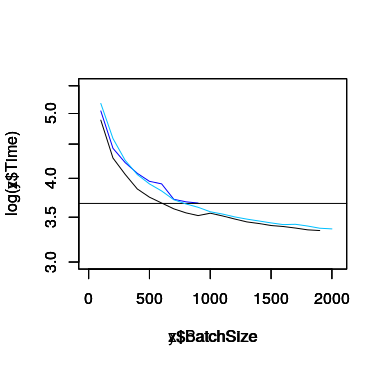
\includegraphics[width=0.8\textwidth]{KapitelPartB/Images/timeVsBatchSize_Amp.png}
 % timeVsBatchSize_Amp.png: 387x367 px, 96dpi, 10.24x9.71 cm, bb=0 0 290 275
 \caption{Vergleich Trainingszeit einer Epoche für verschiedene Optimierungsstufen von Amp Apex. DunkelBlau=O0; Schwarz = O1; Hellblau=O2}
 \label{fig:amp}
\end{figure}
\url{https://developer.download.nvidia.com/video/gputechconf/gtc/2019/presentation/s9998-automatic-mixed-precision-in-pytorch.pdf} zeigt, dass bezüglich der Accuracy kein Verlust zu erwarten ist.

Da O2 gegenüber O1 keinen signifikanten zusätzlichen Gewinn bringt nutze O1.



\subsection{LARS}\label{sec:lars}
\todo[inline]{Experimente fast fertig (3x mal auf einer Graka für 50 min); dann etwa 3 Stunden fürText + Evaluierung}




Es stellt sich die Frage, ob das einen so grossen Einfluss auf die Ausführungszeit hat.



Man sieht, dass mit steigender Batchgröße die Ausführungszeit sinkt. 

Errechne zusätzlich noch ein Modell, wo abhängig von der Modellgrösse währenddem Pruning die Batchgrösse angepasst wird.





\subsection{Beschleunigung der Berechnung des Gradientenabstiegverfahren}
\todo[inline]{ab hier löschen}

Accelerating CNN Training by Sparsifying Activation Gradients funktioniert nur auf Toy-Benchmarks 


\subsubsection{Weight Normalization: A Simple Reparameterization
to Accelerate Training of Deep Neural Networks}


Könnte funktionieren. Code für Lasagne: https://github.com/TimSalimans/weight\_norm


\subsubsection{Accelerating Deep Neural Network Training with Inconsistent Stochastic Gradient Descent}

Interessant bisher kein Code verfügbar

\subsubsection{Accelerated CNN Training Through Gradient Approximation }

Interessant bisher kein Code verfügbar


\end{comment}
